% 
% Author: Bratin Mondal
% Roll No: 21CS10016
% Deparment of Computer Science and Engineering
% Indian Institue of Technology, Kharagpur
%

\documentclass[12pt]{article}
\usepackage{amsmath, amssymb, graphicx}
\usepackage{amsthm}  
\usepackage{float} 
\usepackage{geometry}
\usepackage{hyperref} 
\usepackage{cleveref}
\geometry{a4paper, top=0.25in, bottom=0.25in, left=0.25in, right=0.25in}  

\title{Computational Geometry (CS60064)\\ Homework Set 1}
\author{
    Bratin Mondal - 21CS10016
}
\date{}

\newtheorem{claim}{Claim} 

\begin{document}
\maketitle

\section*{Question 1}
Given \( n \) points on the \(xy\)-plane, design an algorithm to construct a simple polygon \( P \) such that all the given points serve as vertices of \( P \), and no other points are included as vertices.  Provide a proof of correctness for your algorithm and deduce its time complexity. (A \textit{simple polygon} is defined as one in which no two edges intersect, except possibly at their endpoints.) 

\subsection*{Input} Let us denote the set of \( n \) points as \( S = \{s_1, s_2, \ldots, s_n\} \).

\subsection*{Description of the Algorithm}
\begin{enumerate}
    \item From the set \(S\), select the leftmost point with the minimum \(x\)-coordinate. If there are multiple points with the same minimum \(x\)-coordinate, choose the one with the minimum \(y\)-coordinate. Similarly, select the rightmost point with the maximum \(x\)-coordinate. In case of ties, choose the point with the minimum \(y\)-coordinate. Denote these points as \(s_{\text{left}}\) and \(s_{\text{right}}\), respectively.

    \item Define a set \(S' = S \setminus \{s_{\text{left}}, s_{\text{right}}\}\) and initialize two empty sets \(A\) and \(B\). For each point \(s_i \in S'\), determine its position relative to the line joining \(s_{\text{left}}\) and \(s_{\text{right}}\). To do this, compute the vector cross product:
    \[
    (s_{\text{right}} - s_{\text{left}}) \times (s_i - s_{\text{left}}).
    \]
    If the result is positive or zero (indicating that the point lies above or on the line), add \(s_i\) to set \(A\). Otherwise, add \(s_i\) to set \(B\).

    \item Sort the points in set \(A\) in increasing order of \(x\)-coordinates, breaking ties by \(y\)-coordinates (if two points have the same \(x\)-coordinate, the one with the smaller \(y\)-coordinate comes first). Similarly, sort the points in set \(B\) in decreasing order of \(x\)-coordinates, breaking ties by \(y\)-coordinates (if two points have the same \(x\)-coordinate, the one with the larger \(y\)-coordinate comes first).

    \item Form the polygon \(P\) by concatenating the points in the following sequence: \(s_{\text{left}} \rightarrow A \rightarrow s_{\text{right}} \rightarrow B\).
\end{enumerate}

\begin{figure}[H]
    \centering
    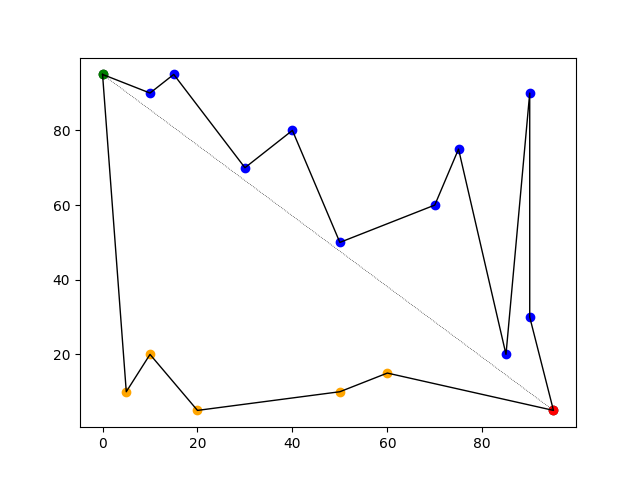
\includegraphics[width=0.5\textwidth]{img/polygon.png}
    \caption{Construction of the simple polygon}\label{fig:polygon}
\end{figure}

The algorithm is illustrated in \Cref{fig:polygon}. The green point represents \(s_{\text{left}}\), and the red point represents \(s_{\text{right}}\). Blue points belong to set \(A\), and yellow points belong to set \(B\). Points in \(A\) lie above or on the line joining \(s_{\text{left}}\) and \(s_{\text{right}}\), while points in \(B\) lie below that line.

\subsection*{Proof of Correctness}

\begin{claim}
    The polygon \(P\) constructed by the algorithm includes all points in \(S\) as its vertices, with no extra points.
    \label{claim1}
\end{claim}

\begin{proof}
    By construction, all points in \(S\) except \(s_{\text{left}}\) and \(s_{\text{right}}\) are partitioned into sets \(A\) and \(B\). In step 4, the final polygon \(P\) is formed by concatenating \(s_{\text{left}}\), the points in \(A\), \(s_{\text{right}}\), and the points in \(B\). This ensures that all points in \(S\) are included as vertices of the polygon and no additional points are added. Hence, the claim holds.
\end{proof}

\begin{claim}
    The polygon \(P\) constructed by the algorithm is simple, meaning that no two edges intersect, except possibly at their endpoints.
    \label{claim2}
\end{claim}

\begin{proof}
    Consider each segment in the output polygon \(P\). We will show that during the construction, any segment added to the polygon does not intersect with any other segment already added.

    We begin with \(s_{\text{left}}\). The first segment added is from \(s_{\text{left}}\) to the first point in set \(A\). Since this is the first segment, it does not intersect with any other segment. As we proceed by increasing \(x\)-coordinates, each new segment is added to the right, while the previous segments are to the left. In the case of two consecutive points having the same \(x\)-coordinate, the point with the smaller \(y\)-coordinate comes first. This guarantees that all previously added segments are either to the left or below the current segment. Thus, as we move from \(s_{\text{left}}\) through set \(A\) to \(s_{\text{right}}\), no intersecting segments are added. We denote these segments as \(L_{1}\).
    
    A similar argument applies when we move from \(s_{\text{right}}\) through set \(B\) to \(s_{\text{left}}\), and we denote these segments as \(L_{2}\).
    
    Finally, segments in \(L_{1}\) and \(L_{2}\) cannot intersect because the segments in \(L_{1}\) lie on or above the line joining \(s_{\text{left}}\) and \(s_{\text{right}}\), while the segments in \(L_{2}\) lie below that line. Therefore, the polygon \(P\) is simple.
\end{proof}

\subsection*{Time Complexity Analysis}
\begin{itemize}
    \item Step 1 requires \(O(n)\) time to find \(s_{\text{left}}\) and \(s_{\text{right}}\).
    \item Step 2 requires \(O(n)\) time to determine the position of each point relative to the line.
    \item Step 3 requires \(O(n \log n)\) time to sort the points in sets \(A\) and \(B\).
    \item Step 4 requires \(O(n)\) time to construct the final polygon.
\end{itemize}

Thus, the total time complexity of the algorithm is \(O(n \log n)\).




\section*{Question 2}

A convex polygon $P$ is provided as a counter-clockwise ordered sequence of $n$ vertices, with their locations specified as $(x, y)$ coordinates. Given a query point $q$, develop an algorithm to determine whether $q$ lies inside $P$ in $O(\log n)$ time, using $O(n)$ space, including any necessary preprocessing. Justify the time and space complexities of your algorithm.

\subsection*{Input}
Let us denote the convex polygon as \(P = \{p_1, p_2, \ldots, p_n\}\) listed in counter-clockwise order and the query point as \(q = (x_q, y_q)\).

\subsection*{Preprocessing}

\begin{enumerate}
    \item Identify the point with the minimum \(x\)-coordinate. If there are ties, choose the point with the maximum \(y\)-coordinate. Arrange the vertices of the polygon in counter-clockwise order starting from this point. Assume, without loss of generality, that the vertex with the minimum \(x\)-coordinate is \(p_1\), and let the ordered vertices be \(P = \{p_1, p_2, \ldots, p_n\}\).
    
    \item For \(i = 3,4, \ldots, n-1\), draw line segments from \(p_1\) to \(p_i\). Since the polygon is convex, the convex angle formed by the line segment \(p_1p_i\) with \(p_1p_2\) strictly increases as \(i\) increases. These line segments divide the polygon into \(n-2\) triangles.
\end{enumerate}

\begin{figure}[h]
    \centering
    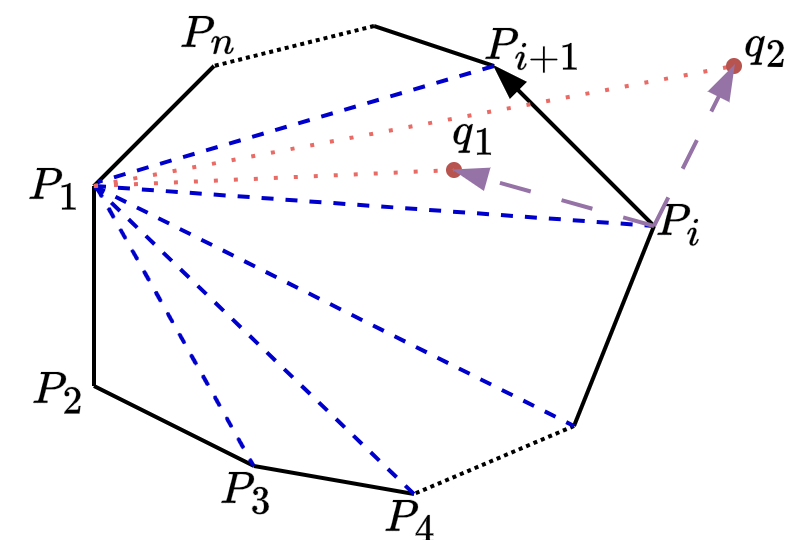
\includegraphics[width=0.5\textwidth]{img/Convex_Polygon.png}
    \caption{Illustration of locating the point \(q\) in the convex polygon}\label{fig:convex_polygon}
\end{figure}

\subsection*{Processing a Query}
\begin{enumerate}
    \item First, check if the query point \(q\) lies inside the convex angle \(p_2p_1p_n\). Any point inside the polygon must also lie inside or on one of the triangles \(p_1p_ip_{i+1}\) for some \(i = 2, 3, \ldots, n-1\). Additionally, the line segment \(p_1q\) must lie within the convex angle \(p_2p_1p_n\).  

    To verify this, compute the cross products:
    \[
    (p_2 - p_1) \times (q - p_1) \quad \text{and} \quad (p_n - p_1) \times (q - p_1).
    \]
    For the point \(q\) to lie inside the convex angle, the first cross product must be non-negative, and the second cross product must be non-positive.  

    If this condition is not satisfied, \(q\) lies outside the polygon. Otherwise, proceed to the next step.

    \item To find the triangle in which the query point \(q\) potentially lies, perform a binary search. Assume that \(q\) lies in the triangle \(p_1p_ip_{i+1}\). In this case:
    \[
    (p_1p_j) \times (p_1q) \geq 0 \quad \text{for } j \leq i, \quad \text{and} \quad (p_1p_j) \times (p_1q) < 0 \quad \text{for } j > i.
    \]
    Using this property, perform a binary search to find the maximum \(i\) such that:
    \[
    (p_1p_i) \times (p_1q) \geq 0.
    \]
    Denote this value as \(i_{\text{max}}\).

    \item After identifying \(i_{\text{max}}\), determine if the query point lies inside the polygon.  

    If \(i_{\text{max}} = n\), then \(p_1p_n\) and \(p_1q\) are collinear. To check if \(q\) lies on the line segment \(p_1p_n\), compare the length of \(p_1p_n\) with the sum of the lengths of \(p_1q\) and \(qp_n\). If the lengths are equal, \(q\) lies on \(p_1p_n\) and hence inside the polygon. Otherwise, \(q\) lies outside.  

    If \(i_{\text{max}} < n\), then the query point potentially lies inside the triangle \(p_1p_{i_{\text{max}}}p_{i_{\text{max}}+1}\). To verify this, compute the cross product:
    \[
    (p_{i_{\text{max}}+1} - p_{i_{\text{max}}}) \times (q - p_{i_{\text{max}}}).
    \]
    If the cross product is non-negative, \(q\) lies inside the triangle. Otherwise, \(q\) lies outside the polygon. (In \Cref{fig:convex_polygon}, point \(q_1\) lies inside the triangle \(p_1p_ip_{i+1}\), while point \(q_2\) lies outside the polygon.)
\end{enumerate}

\subsection*{Time Complexity Analysis}

\subsubsection*{Preprocessing}
 Preprocessing requires \(O(n)\) time to find the minimum \(x\)-coordinate and arrange the vertices in counter-clockwise order. Joining the vertices to form triangles requires \(O(n)\) time since we join \(n-3\) line segments. Note that computing the segments can either be done once during preprocessing or on the fly during query processing.

\subsubsection*{Processing a Query}
\begin{itemize}
        \item Step 1 requires \(O(1)\) time to compute the cross products for determining if the query point lies inside the convex angle.
        \item Step 2 requires \(O(\log n)\) time to perform a binary search to find \(i_{\text{max}}\).
        \item Step 3 requires \(O(1)\) time to verify if the query point lies inside the polygon.
\end{itemize}

Since the binary search dominates the time complexity, the overall time complexity of the algorithm is \(O(\log n)\).

\subsection*{Space Complexity Analysis}
The space complexity of the algorithm is \(O(n)\) for storing the vertices of the polygon. Additionally, the newly added line segments require \(O(n)\) space. However, it's important to note that the segment information is redundant and can be computed on the fly. Since the input vertices are already provided, they require \(O(n)\) space, and no extra space is used for storage. Therefore, the overall space complexity remains \(O(n)\).


\end {document}